%for reference to this section
\section{Einleitung}
\label{section:Introduction}

In der Medizinischen Forschung ist es wichtig, dass Studienergebnisse mit 
fehlenden Daten sorgfältig analysiert und bearbeitet werden. Das soll verhindern, dass es zu einer Verzerrung des 
Ergebnisses kommt. Viele Medizinische Zeitschriften verlangen bereits einen korrekten Umgang mit Fehlenden Daten sowie 
eine Rechtfertigung für den gewählten statistischen Ansatz. \autocite[163]{Lee2014} 
Eine wichtige Methode zur Behandlung von fehlenden Daten ist die Multiple Imputation (MI).

Die Multiple Imputation (MI) ist ein statistisches Verfahren, in welchem fehlende Daten anhand einer 
Wahrscheinlichkeitsverteilung mehrfach ersetzt und gemittelt werden. \autocite[163]{Lee2014}

Ziel dieser Arbeit ist es, einen Überblick über die MI im Medizinischen Bereich zu geben. Neben einer 
Erklärung der MI, wird auf wichtige Fragestellungen bei der Durchführung der MI eingegangen.

Ein wichtiger Teil bei der Durchführung der MI ist die Planung der MI und die Überprüfung des Datensatzes. 
Dabei wird im Forschungsblatt der Anteil von fehlenden Daten sowie die Art der fehlenden Daten erläutert. 
Des Weiteren muss die Methode der Imputation gewählt werden. Es werden einige Alternativen zur MI aufgezeigt und es 
wird auf den Vorteil von Hilfsvariablen bzw. Post-Baseline Untersuchungen eingegangen. Nach der Durchführung der Imputation 
kann die Sensitivität/Qualität ermittelt werden. Hierbei werden im Forschungsblatt unterschiedliche Mittel zur 
Qualitätsfeststellung beschrieben.


\section{Multiple Imputation}
\label{section:MI}

\subsection{Anwendungsbeispiel der MI}

Angenommen es würde eine Studie über den Zusammenhang zwischen Blutdruck und dem Risiko eines Herzinfarkts geben. 
Dabei fehlen die Blutdruck Daten bei einigen Herzinfarkt-Patienten. Man kann nun aufgrund der anderen Daten die 
gesammelt wurden Rückschluss auf die fehlenden Daten ziehen. So können z.B. die fehlenden Blutdruck-Daten einiger 
Patienten ersetzt werden, indem andere Patienten mit gleichen Eigenschaften gesucht werden. Bei Patienten mit gleichen 
Eigenschaften (z.B. gleiches Alter, gleicher BMI) steigt auch die Wahrscheinlichkeit, dass der Puls-Wert ähnlich ist. 

Allerdings kann diese Vorgehensweise aufwändig werden. Vor allem, wenn es sehr viele Variablen gibt. Es wird z.B. 
schwierig werden, einen Patienten mit genau dem selben BMI, Alter, Blutdruck, Geschlecht etc. zu finden. Daher wird in 
der MI versucht, anhand der vorhandenen Daten und einer Verteilungsfunktion eine Vermutung über den fehlenden Wert zu 
bekommen. Man könnte z.B. davon ausgehen, dass die Pulswerte der Bevölkerung Normalverteilt sind. Aufgrund dieser Vermutung 
kann der Mittelwert aller Pulswerte gebildet und für die fehlenden Daten eingesetzt werden. Für Komplexere Sachverhalte ist 
dieses Vorgehen allerdings nicht ausreichend. \autocite[1089]{Donders2006}

Um den gesamten Sachverhalt besser darstellen zu können, werden z.B. mehrere voneinander abhängige Regressionsmodelle 
(Conditional Regression Models) oder eine Mehrdimensionale Normalverteilung (Joint Normal Distribution) benötigt. Damit 
werden mehrere Eigenschaften/Variablen berücksichtigt. \autocite[164]{Lee2014}.  Aus so einem Modell werden die 
Werte nun nicht nur einmal, sondern mehrfach imputiert. Für die Studie könnte z.B. ein Conditional Regression Modell erstellt 
werden, dass das Risiko eines Herzinfarktes bezogen auf Alter, Blutdruck, BMI, etc. darstellt. Werden nun aus diesem 
Regressions Modell mehrfach Schätzwerte gezogen und diese Schätzwerte dann kombiniert, handelt es sich um eine MI. 

\subsection{Funktionsweise der MI}

Ausgangspunkt der MI ist das Analysis Modell. Das Analysis Modell ist ein Datensatz, in welchem Daten verschiedener Variablen 
fehlen können. In der ersten Phase der MI wird aus dem Analysis Modell ein Imputation Modell erstellt. Dazu werden dem 
Analysis Model noch zusätzliche Variablen, sogenannte auxiliary variables (Hilfsvariablen) hinzugefügt. Die fehlenden 
Daten werden darauf hin z.B. mit Hilfe eines Regressionmodells mehrfach imputiert. Durch die mehrfache Imputation enstehen 
mehrere Vervollständigte Datensätze. In der zweiten Phase werden die Vervollständigten Datensätzte analysiert und gemittelt, 
wodurch der finale Datensatz ermittelt wird. Durch die Berechnung des Standard Errors kann die Unsicherheit der Daten 
ermittelt werden. \autocite[163]{Lee2014} Im Folgenden wird auf die beiden Phasen der MI näher eingegangen.

\subsection{Phase 1: Mehrfache Imputation}

Die Grundsätzliche Idee der MI ist es, ein Regressionsmodell zu erstellen, dass mögliche Werte für die zu ersetzenden Werte 
beinhaltet. Aus diesem Regressionmodell werden in Folge anhand einer Simulation randomisiert Werte gezogen. Angenommen, es 
würde sich um eine Normalverteilung handeln, dann würden die fehlenden Daten vereinfacht über folgende Formel aus \textcite[8]{Enders2017} gezogen werden:
\begin{equation}
 Y_{(mis)}\sim N(\widehat{Y}, \sigma_\varepsilon^2)
\end{equation}
„$Y_{(mis)}$ ist ein Schätzwert für den fehlenden Wert. $\sim N$ bezeichnet die Normalverteilung, $\widehat{Y}$ ist der vorhergesagte Wert aus 
einer Regressionsgleichung und $\sigma_\varepsilon^2$ ist die Residuenvarianz aus der Regression.“ \autocite[8]{Enders2017}  Die Varianz definiert 
den Mittelwert sowie die Streuung. Insgesamt ist die Imputation aus einer Gleichung die Summe eines Abweichungswertes 
(Varianz) und des vorhergesagten Wertes. \autocite[8]{Enders2017} Um fehlende Daten in mehreren Variablen zu brücksichtigen 
werden komplexere Regressionsmodelle, wie das Conditional Regression Model oder die Joint Normal Distribution benötigt. 
Das Zufällige ziehen von Schätzungen zu den fehlenden Werten wird mehrfach wiederholt, wodurch mehrere Vollständige 
Datensätze entstehen, auf denen daraufhin die Analyse durchgeführt wird. \autocite[163 ff.]{Lee2014} Durch das 
wiederholen der Imputationen mit unterschiedlichen, plausiblen Regressions-Parametern, gleichen die Datensätze keiner 
Imputation der anderen. Dadurch wird die Unsicherheit der Imputation addressiert. \autocite[8]{Enders2017}

\subsection{Phase 2: Analyse der Daten}

In der 2. Phase wird jeder der Imputierten Datensätze getrennt Betrachtet. Wenn z.B. 20 Imputationen durchgeführt wurden, 
gibt es 20 Datensätzte, die Schätzwerte für die fehlenden Werte beinhalten. Für jeden dieser Datensätze wird ein gemeinsamer 
Schätzwert (z.B. über das Arithmetische Mittel) und der Standard Error berechnet. Zuletzt werden die 20 Datensätze noch 
kombiniert, indem das Arithmetische Mittel der Schätzwerte sowie des Standart Errors gebildet wird. \autocite[10]{Enders2017}

\subsection{Praktische Anwendung der MI}

Statistische Programme wie SAS und Stata unterstützen bereits MI unter der Verwendung des Contitional Regression Modells 
sowie der Joint Normal Distribution. \autocite[164]{Lee2014}. Da dieses Paper einen Allgemeinen Überblick über die MI 
geben soll, wird auf die genaue Implementation nicht mehr eingegagnen. 

Eine Implemetation der MI kann in \textcite[]{Royston2005} gefunden werden. Dort wird die Implementierung der MI in der MICE Methode 
näher anhand von ado-Dateien erläutert. Ado-Dateien sind Dateien, welche vom Statistik Programm Stata vewendet werden.

\subsection{Vorgehensweise MI}

Bevor die MI durchgeführt werden kann. Sollten einige wichtige Punkte geklärt werden, die in den nächsten 
Kapiteln näher erläutert werden. So stellt sich unter anderem die Frage, wie groß der Anteil an fehlenden 
Daten ist und welche Auswirkungen dies hat. (Siehe Kapitel \ref{section:missing_data}). Nach der 
Durchführung der MI sollte zu dem die Qualität der MI überprüft werden (siehe Kapitel \ref{section:qualtity}).


\section{Anteil an fehlenden Daten}
\label{section:missing_data}

Es gibt in der Forschung unterschiedliche Empfehlungen, bis zu welchem Anteil an fehlenden 
Daten zuverlässige Ergebnisse erzielt werden können. Statistische Leitartikel gehen davon aus, 
dass es ab 10\% an fehlenden Daten wahrscheinlich zu einem Bias kommen kann. Ab 40\% sollte 
das Ergebnis der MI nur mehr als Hypothese gesehen werden. Die Beweislage, die diese Grenzen 
stützt, ist allerdings gering. \autocite[63 f.]{Madley-Dowd2019}

In der Studie “The proportion of missing data should not be used to guide decisions on multiple imputation” wird 
argumentiert, dass der Anteil an fehlenden Daten nicht unbedingt ausschlaggebend für den Erfolg oder Misserfolg der 
MI steht. Viel mehr spielen die Art der fehlenden Daten und die Verwendung von auxilliary Variablen eine wichtige Rolle. 

\section{Art der fehlenden Daten}
\label{section:descriptor_of_missingness}

Nach Definition von (Little \& Rubin, 2002; Rubin, 1976) gibt es 3 verschiedene Arten von fehlenden Daten:

\subsection{MCAR: Missing Completely at Random}

Die Fehlenden Daten haben keine Verbindung zu den zu analysierenden Daten. Gründe für MCAR Daten 
können zum Beispiel ein Strom- oder Internetausfall sein. \autocite[8]{Enders2017}

\subsection{MAR: Missing at Random}

Systematische Unterschiede zwischen den fehlenden Daten und den Untersuchten Daten können erklärt 
werden. So können zum Beispiel Blutdruckwerte v.a. bei jüngeren Personen fehlen, da bei diesen 
der Blutdruck weniger oft kontrolliert wird. \autocite[157]{Sterne2009} An den vorhandenen Daten 
kann man nun erkennen, dass es bei Menschen mit Jüngerem Alter öfter zu fehlenden Blutdruckdaten 
kommt. Man könnte daher repräsentativ für die fehlenden Blutdruckdaten, die Blutdruckdaten anderer 
Junger Teilnehmer verwenden, bei welchen die Messung des Blutdrucks nicht vergessen wurde. 

\subsection{NMAR: Not Missing at Random}

Es gibt systematische Unterschiede, welche nicht anhand der Untersuchten Daten erkannt werden 
können. NMAR Daten können zum Beispiel entstehen, wenn Patienten mit hohem Blutdruck häufiger 
aufgrund von Kopfschmerzen fehlen. \autocite[157]{Sterne2009} Anhand der vorhandenen Daten kann
 man nun nicht erkennen, dass es eine Gruppe von Menschen mit Kopfschmerzen gibt, welche bei den 
 Blutdruckmessungen fehlt. 

NMAR-Daten können anhand von statistischen Tests nicht identifiziert werden. NMAR-Daten können 
also nur als solche durch vorhandenes Wissen interpretiert werden. Daher gibt es keine allgemein 
Gültige Methode für die Behandlung von NMAR-Daten. \autocite[1088]{Donders2006}

\subsection{Auswirkungen auf das Ergebnis der MI}

MAR- und NMAR Daten sind schwer zu unterscheiden. NMAR können jedoch zu einem voreingenommenen Resultat führen.  Um das 
Risiko eines voreingenommenen Ergebnisses durch NMAR Daten zu verringern, kann eine Sensitivitätsanalyse angewendet 
werden. \autocite[157]{Sterne2009} 

Wenn es sich um MCAR Daten handelt, können anstatt der MI einfachere Methoden wie die Complete Case Anlaysis in Betracht 
gezogen wereden. \autocite*[1088]{Donders2006} 

\section{Alternativen zur MI}
\label{section:alternatives}

\subsection{Complete Case Analysis (CCA)}

Bei der CCA werden Teilnehmer mit fehlenden Daten aus der Studie exkludiert. \autocite[3]{Jakobsen2017} 

In einer Simulation aus \textcite[]{VanderHeijden2006} erzielte die CCA schlechtere Ergebnisse als die MI. Für 
die Simulation wurden Daten aus einer Studie zu Lungenembolie mit 398 Subjekten verwendet. Dabei gab es 
einen Unterschiedlichen Anteil an fehlende Daten bei einigen Variablen. Bei den fehlenden Daten handelte es 
sich nicht um MCAR Daten.  Das Ergebnis der CCA schnitt dabei in allen Messgrößen im Vergleich zur single- 
und multiplen Imputation schlechter ab. Als Qualitätskriterien wurden u.a. der Standard Error sowie die 
Regressions Koeffizienten verwendet. Mögliche Qualitätskriterien werden in Kapitel XY nochmals näher erläutert.

Wenn es sich im Datensatz wie in der oben genannten Simulation nicht um MCAR-Daten handelt, dann ist das Ergebnis der 
CCA vermutlich voreingenommen. Grund dafür ist, dass die CCA systematische Unterschiede nicht 
berücksichtigt. \autocite[157]{Sterne2009} Im Fall von MAR-Daten eignet sich daher die Single- oder Multiple 
Imputation Imputation besser. \autocite[1088]{Donders2006}


\subsection{Single Imputation}

Bei der Single Imputation werden fehlende Daten nach einer Regel ersetzt. Von der Single Imputation gibt es mehrere 
Varianten. Bei der Last Observation Carried Forward (LOCF) werden fehlende Daten mit den Daten aus der letzten 
Untersuchung ersetzt. Bei der Worst Observation Carried Forward werden fehlende Daten mit dem schlechtesten untersuchten 
Ergebnis des Patienten ersetzt. Bei der Simple Mean Imputation wird der Mittelwert verwendet. Die Single Imputation hat 
die Annahme, dass fehlende Werte und in der Vergangenheit gemessene Werte identisch sind. Diese Annahme ist allerdings 
unrealistisch, weshalb diese Methode mit Bedacht eingesetzt werden soll.
\autocite[3]{Jakobsen2017}

Eine Simulation aus \textcite[]{Young-Saver2018} zeigt, dass mit der LOCF Methode ähnlich gute oder sogar bessere 
Ergebnisse erzielt werden können als mit der MI. In der Simulation wurden Daten aus einer Studie zu akutem Schlaganfall 
verwendet. Begründet wird das gute Abschneiden der LOCF u.a. mit der zeitlichen Nähe der letzten Untersuchung zu dem zu 
schätzen den Wert. Durch die zeitliche Nähe haben zeitrelevante Prozesse, wie Neuroplastizität oder Neuronale Regeneration 
(neuronale Prozesse) keinen so großen Einfluss. Zudem ist die Wahrscheinlichkeit von Vorfällen geringer, welche Einfluss 
auf die zu erhebenden Werte haben könnten. Dazu gehören z.B. Unfälle oder Herzinfarkte. \autocite[3667]{Young-Saver2018}. 
Wie gut die LOCF Methode im Vergleich zur MI abschneidet kann jedoch nicht allgemein gesagt werden und hängt maßgeblich 
von den verwendeten Daten ab. 


\subsection{Wann bietet sich der Einsatz von CCA oder Single Imputation an?}

Die Anwendung der CCA bietet sich an, wenn es sich um MCAR-Daten handelt. 
Die Single Imputation sollte mit Bedacht eingesetzt werden. Sie kann jedoch unter Umständen ähnliche gute Ergebnisse 
wie die MI erzielen. Die LOCF Methode bietet sich vor allem an, wenn es relevante, zeitnahe Untersuchungen gibt und es 
sich bei den untersuchten Variablen um Zeitrelevante Prozesse handelt. 


\section{Zusätzliche Daten}
\label{section:additional_data}

\subsection{Post-Baseline Untersuchungen}

Die Simulation aus \textcite[]{Young-Saver2018} zum Thema akutem Schlaganfall, welche im Kapitel „Single Imputation“ 
bereits erwähnt wurde, zeigt auch die Bedeutung von Post-Baseline Untersuchungen. Post-Baseline Untersuchungen sind
 Untersuchungen, die nach einem Bestimmtem Ereignis erhoben wurden. Im Falle der Studie wurde der NIH Stroke Scale 
 nach 24 Stunden und der mRS nach 7-10 Tagen erhoben. (der NIH Stroke Scale und der mRS sind beides Bewertungskalen
  für die Symptome des Patienten). Die MI wurde einmal mit und einmal ohne Daten aus den Post-Baseline Untersuchungen 
  durchgeführt. Im Ergebnis der Simulation schnitt die Multiple Imputation mit Post-Baseline besser ab als ohne (siehe Abbildung \ref{figure:study})

  \begin{figure*}[t]
	\centering
	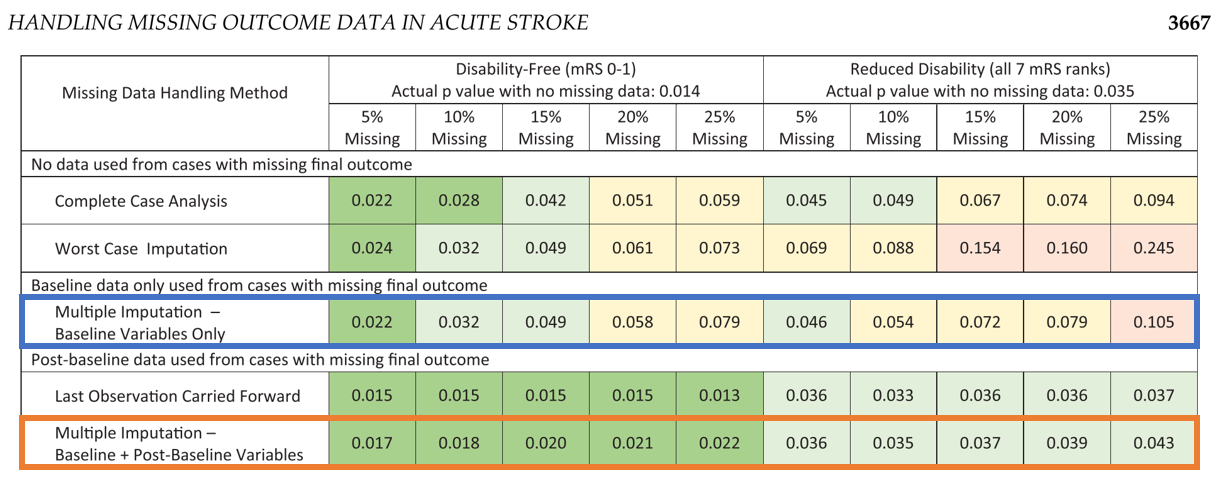
\includegraphics[width=0.9\textwidth]{images/grafik_saver.png}
	\caption{
		Die MI mit Post-Baseline Variablen (orange umrahmt) schnitt bei jedem Prozentsatz an fehlenden Daten besser ab als 
		die MI ohne Post Baseline Variablen (blau umrahmt). Berechnet wurde der P-Value. Je näher der P-Value an 1 liegt, 
		desto höher ist die Wahrscheinlichkeit, dass die Ergebnisse Zufall sind. Ein niedriger P-Value ist daher anzustreben. 
		Grafik aus \textcite[3667]{Young-Saver2018}, die Beschriftung sowie die blaue/orange Markierung wurde nachträglich 
		hinzugefügt.
	}
	%for reference to this figure
	\label{figure:study}
\end{figure*}


\subsection{Hilfsvariablen}

Unter Hilfsvariablen (engl.: auxiliary variables) versteht man Variablen, welche dem Datensatz im Nachhinein hinzugefügt werden, 
um die Menge an Information zu erhöhen. Auxilliary Variablen können z.B. aus anderen Studien/Datensätzen 
herangezogen werden.

Eine Simulation in \textcite[]{Madley-Dowd2019} zeigt die Bedeutung der Auxilliary Variablen. 
Die Simulation wurde anhand von Daten aus ALSPAC (Avon Longitudinal Study of Parents and Children) 
durchgeführt.


\section{Qualitätsfeststellung MI}
\label{section:qualtity}

\subsection{Bias}

Ein Qualitätskriterium für die MI ist der Bias. Unter Bias versteht man einen systematischen Fehler. Dieser Fehler entsteht, 
wenn der Einfluss von Eigenschaften über- oder unterbewertet wird. \autocite[2]{Jakobsen2017} Angenommen, der Blutdruck 
ist ein wichtiger Faktor bei der Entstehung von Herz-Kreislauferkrankungen. Sollte eine Studie den Blutdruck nicht als Faktor 
für die Entstehung von Herz-Kreislauferkrankungen miteinbeziehen, ist das Ergebnis vermutlich biased bzw. voreingenommen.

Eine ordnungsgemäße Durchführung der MI, sowie eine genaue Überprüfung des Datensatzes, ist noch keine Garantie dafür, 
dass das Ergebnis nicht biased ist. Vor allem wenn nicht klar ist, ob es sich bei den verwendeten Daten um MAR oder MNAR 
Daten handelt. Es gibt einige Möglichkeiten, um die Qualität der MI zu Überprüfen und damit auch eine Abschätzung über einen 
Möglichen bias zu geben. Im Folgenden werden diese 

\subsection{Standard Error und P-Value}

Standardmäßig wird in der MI der Standard Error berechnet. Der Standarderror ist ein Maß für die Unsicherheit der 
geschätzten Werte. \autocite[1098]{Donders2006} 

Des Weiteren kann der P-Wert berechnet werden. Der P-Wert ist ein Wert zwischen 0 und 1. Je höher der P-Wert ist, 
desto höher ist die Wahrscheinlichkeit, dass die Ergebnisse Zufall sind. Ein niedriger 
P-Wert ist in der MI daher anzustreben. 


\subsection{Simulierte fehlende Daten}

Eine einfache Methode zur Qualitätsüberprüfung ist es, einen vollständigen Datensatz zu nehmen und die fehlenden Daten zu 
simulieren. Nach dieser Vorgehensweise wurde auch die Simulation aus (D. Young-Saver, 2018) durchgeführt. Hierbei wurde 
aus dem Vollständigen Datensatz auf Basis eines randomisierten Verfahrens Daten gelöscht. Daraus folgt, dass man nun die 
imputierten Daten mit den Daten des Vollständigen Datensatzes vergleichen kann. Ein möglicher Vergleich wäre z.B. die 
Bestimmung der exakten Übereinstimmungsrate. Hierbei wird der Anteil von exakten Übereinstimmungen zwischen den imputierten 
und originalen Werten bestimmt. Des Weiteren kann Spearmans Korrelationskoeffizient, oder die Mittlere (Absolute) Abweichung 
bestimmt werden. \autocite[3664]{Young-Saver2018} 

\subsection{Sensitivitätsanalyse}

Vor der Durchführung der MI sollte eine Vermutung über die Art der fehlenden Daten gemacht werden. Sind die Daten MAR, MNAR 
oder MCAR? Angenommen es gibt eine Studie, die den Zusammenhang zwischen Blutdruck und Herz-Kreislauferkrankungen untersucht. 
Sllte ein Teil der Patienten diese Studie vorzeitig verlassen, könnte man vermuten, dass dies komplett zufällig geschieht. 
Die Daten wären somit MCAR. Es könnte aber auch sein, dass einige Patienten die Studie aufgrund von Kopfschmerzen wegen zu 
hohen Blutdrucks verlassen. Damit gäbe es einen systematischen Zusammenhang und die Daten währen MAR oder MNAR. In vielen 
Studien ist es schwer, eine sichere Vermutung über die Art der fehlenden Daten zu treffen. Mit Sensitivitätsanalysen können 
mehrere Vermutungen über die Art der fehlenden Daten überprüft werden. \autocite[2815]{Cro2020} (Cro, Suzie, 2020)

Im Allgemeinen gibt es 2 Varianten der Sensitivitätsanalyse: $\delta$-basiert und referenzbasiert. In der $\delta$-basierten Variante 
wird dem zu Erwarteten Wert noch ein Offset Variable $\delta$(Delta) hinzugefügt, welche den Einfluss von 
fehlenden/nicht-beobachteten Teilnehmern bewertet.  In der Referenzbasierten Sensitivitätsanalyse werden Werte aus 
anderen Gruppen des Versuchs imputiert, welche Referenz zu den Beobachteten Werten beinhaltet. \autocite[2815]{Cro2020} 
Eine praktische Beschreibung der Durchführung der Sensitivitätsanalyse in Verbindung mit der MI kann in 
\textcite[]{Cro2020} gefunden werden.

\section{Fazit}

Eine sorgfältige Planung und Durchführung der Imputation ist wichtig, damit es nicht zu verzerrten Ergebnissen kommt. 
Im ersten Schritt sollte der verwendete Datensatz überprüft werden. Bei den Verwendeten Daten sollte der Anteil an fehlenden 
Daten nicht zu hoch sein. In der Forschung gibt es jedoch Unterschiedliche Vorgaben, welche Menge an fehlenden Daten in 
Ordnung ist. Mehr Forschung wäre hier von Vorteil. Bei der Art der fehlenden Daten sollte es sich möglichst um MAR Daten 
handeln. 

Im Zweiten Schritt sollte die zu verwendende Imputations-Methode, sowie die Verwendung von zusätzlichen Variablen geplant 
werden. 
Handelt es sich um MCAR Daten, kann der Einsatz einer CCA überlegt werden. Gibt es relevante, zeitnahe Untersuchungen 
zu den fehlenden Daten, kann auch die Verwendung der Single Imputation in der LOCF-Variante gute Ergebnisse erzielen. 
Das Hinzufügen von Post-Baseline Untersuchungen oder Auxilliary Variablen kann das Resultat der MI verbessern. 

Nach der Durchführung der MI ist es zu empfehlen, eine Sensitiviätsanalyse durchzuführen. Vor allem, wenn es sich nicht 
sicher um MAR Daten handelt. Der Standard Error sowie der P-Value sollten nicht zu hoch sein, da hohe Werte auf ein 
biased Ergebnis hinweisen könnten.

MI ist eines der wichtigsten Werkzeuge für die Behandlung von fehlenden Daten in vielen verschiedenen Bereichen. 
Wer sich z.B. mit Statistik oder AI beschäftigt, sollte einen Überblick über MI haben. MI ist ein komplexes Thema und 
auch dieses Forschungsblatt konnte nur einen kleinen Überblick zum Thema MI geben. Es ist daher von Vorteil, dass die 
meisten Statistischen Programme bereits MI unterstützen und so den Einstieg in die MI vereinfachen. 


